% Self-contained source. Compile with: latexmk -pdf pde_aware_fem_guide.tex
% Alternatively: pdflatex pde_aware_fem_guide.tex (run twice).
% No external figures, bibliography database, or shell escape required.
\documentclass[11pt,a4paper]{article}
\usepackage[T1]{fontenc}
\usepackage{lmodern}
\usepackage[margin=25mm,headheight=14pt]{geometry}
\usepackage{amsmath,amssymb,mathtools}
\usepackage{booktabs,longtable,array,tabularx}
\usepackage{xcolor,microtype,enumitem,fancyhdr}
\usepackage{tikz,pgfplots}
\usetikzlibrary{arrows.meta,positioning}
\pgfplotsset{compat=1.18}
\usepackage[hyphens]{url}
\usepackage[colorlinks=true,linkcolor=blue!45!black,citecolor=blue!45!black,urlcolor=blue!45!black]{hyperref}
\definecolor{ink}{RGB}{27,49,73}
\definecolor{accent}{RGB}{14,102,111}
\definecolor{pale}{RGB}{239,246,246}
\pagestyle{fancy}
\fancyhf{}
\fancyhead[L]{\small\textcolor{ink}{PDE-aware finite element methods}}
\fancyhead[R]{\small Study guide}
\fancyfoot[C]{\thepage}
\setlength{\parindent}{0pt}
\setlength{\parskip}{6pt}
\setlength{\emergencystretch}{3em}
\setlist[itemize]{leftmargin=*,itemsep=2pt,topsep=3pt}
\setlist[enumerate]{leftmargin=*,itemsep=3pt,topsep=3pt}
\newcolumntype{Y}{>{\raggedright\arraybackslash}X}
\newcolumntype{P}[1]{>{\raggedright\arraybackslash}p{#1}}
\newcommand{\R}{\mathbb{R}}
\newcommand{\dd}{\,\mathrm{d}}
\newcommand{\norm}[1]{\left\lVert #1\right\rVert}
\newcommand{\abs}[1]{\left\lvert #1\right\rvert}
\newcommand{\ip}[2]{\left(#1,#2\right)}
\newcommand{\decision}[1]{\par\smallskip\noindent\textcolor{accent}{\textbf{Consequence for your engine.}} #1\par}
\newcommand{\guarantee}{\textcolor{accent}{\textbf{Mathematical result.}} }
\newcommand{\evidence}{\textcolor{accent}{\textbf{Empirical evidence.}} }
\newcommand{\heuristic}{\textcolor{accent}{\textbf{Practical heuristic.}} }
\hypersetup{pdftitle={Using PDE structure to choose finite element methods},pdfauthor={Prepared for Dmytro Glushko}}

\begin{document}
\hypersetup{pageanchor=false}
\begin{titlepage}
\vspace*{16mm}
{\small\textcolor{accent}{COMPUTATIONAL ENGINEERING / RESEARCH STUDY GUIDE}}\par
\vspace{9mm}
{\Huge\bfseries\color{ink}Using PDE structure\\to choose finite\\element methods\par}
\vspace{8mm}
{\Large Analysis, mesh adaptation, approximation spaces,\\time integration, and efficient solvers\par}
\vspace{12mm}
\rule{\textwidth}{0.6pt}\par
\textbf{Purpose.} Understand how to build a reliable engine for scalar second-order PDEs on prescribed two-dimensional geometries, including time-dependent problems. The emphasis is on methods and their mathematical and empirical justification, with established software used as evidence of implementation practice.

\textbf{Central claim.} There is no reliable rule of the form ``identify the PDE type, then select the best mesh and solver.'' The useful workflow combines operator analysis, boundary and interface data, solution-dependent error estimation, and measured cost at a specified accuracy.

\textbf{Reader assumptions.} Undergraduate engineering mathematics, basic FEM assembly, and ordinary differential equation integration. Standard definitions are kept short; attention goes to assumptions, failure modes, and decisions that change numerical performance.
\vfill
Prepared for Dmytro Glushko\par
Research checked: 30 September 2026\par
\small Primary papers, university notes, and official technical documentation. This is a focused synthesis, not an exhaustive literature survey or a claim that every industrial code follows the same policy.
\end{titlepage}
\hypersetup{pageanchor=true}

\section*{How to use this document}
\addcontentsline{toc}{section}{How to use this document}
Read Sections~\ref{sec:scope}--\ref{sec:spaces} first. They explain what can be inferred from an equation and what must be specified separately. Sections~\ref{sec:mesh}--\ref{sec:nonlinear} connect that information to numerical choices. Section~\ref{sec:empirical} separates published experimental findings from guarantees. Sections~\ref{sec:cases}--\ref{sec:roadmap} turn the material into experiments for your engine.

Statements are marked as \emph{mathematical results}, \emph{empirical evidence}, or \emph{practical heuristics} when the distinction affects a decision. The worked derivations and the one-dimensional experiment are original explanatory calculations. Citations identify the underlying methods and externally reported findings. No universal speedups, universal mesh thresholds, or unconditional adaptivity guarantees are implied.

\textbf{The most important corrections to the initial project idea:}
\begin{enumerate}
\item The PDE normally changes the \emph{discretization of a geometry}, not the physical geometry. Geometry changes require a separate model, such as a moving boundary or shape optimization.
\item ``Second order'' does not specify a numerical method. It includes coercive diffusion, indefinite Helmholtz problems, transport-dominated equations, waves, nonlinear and degenerate problems, and systems with constraints.
\item Mesh refinement and solver choice are coupled. A mesh that reduces approximation error may make the linear system harder or force much smaller explicit time steps.
\item Many effective choices require a preliminary solution. Coefficients predict possible layers; the actual source, boundary conditions, and solution determine which features occur.
\item Efficiency means \emph{time and memory to obtain a sufficiently accurate answer}, not time per iteration, element count, or an attractive solution plot.
\end{enumerate}
\tableofcontents
\clearpage

\section{Define the supported problem before choosing algorithms}\label{sec:scope}
\subsection{A useful first family}
For a fixed domain $\Omega\subset\R^2$, begin with
\begin{equation}\label{eq:family}
\rho_2 u_{tt}+\rho_1 u_t
-\nabla\cdot(D\nabla u)+\boldsymbol\beta\cdot\nabla u+\sigma u=f.
\end{equation}
Here $D$ is a diffusion or stiffness tensor, $\boldsymbol\beta$ a drift field, and $\sigma$ a reaction coefficient. The coefficients may depend on position and time. Later they may depend on $u$. Units need not be those of heat transfer: different physical models give different meanings to the same operator structure.

This family contains stationary diffusion when $\rho_1=\rho_2=0$, heat-like evolution when $\rho_1>0$ and $\rho_2=0$, and wave-like evolution when $\rho_2>0$. It is a useful numerical scope, not all second-order PDEs. It excludes, for example, a general fully nonlinear equation $F(x,u,\nabla u,\nabla^2u)=0$, arbitrary mixed space-time derivatives, and coupled vector constraints.

Boundary conditions, initial data, coefficient interfaces, and a desired output are part of the problem. Two copies of the same differential expression can require very different meshes if these data differ.

\subsection{Divergence and non-divergence form are different inputs}
For sufficiently differentiable coefficients,
\begin{equation}
-\nabla\cdot(D\nabla u)
=-\sum_{i,j}D_{ij}\partial_{ij}u
-\sum_j\left(\sum_i\partial_iD_{ij}\right)\partial_j u.
\end{equation}
Consequently, converting $-D:\nabla^2u$ into a divergence-form operator changes the first-order term unless the coefficient derivatives vanish. At coefficient jumps this classical calculation is unavailable. The weak interface conditions must be derived from the intended model.

Non-divergence equations can need dedicated approaches: mixed Hessian formulations, non-variational FEM, least-squares methods under additional hypotheses, or monotone approximations for viscosity solutions. Parsing an arbitrary differential expression and integrating it by parts is not a sufficient general solution. Least-squares FEM is a substantial alternative methodology with its own norm, boundary, and conditioning issues~\cite{bochev}.

\decision{Use a documented divergence-form scalar family first. Require explicit boundary and initial data, coefficient regions, and supported sign assumptions. Report unsupported structure instead of silently applying a diffusion solver.}

\section{What analysis is possible before solving?}\label{sec:analysis}
\subsection{Principal symbol: classify the highest derivatives}
For a scalar equation in two independent variables,
\begin{equation}
a u_{xx}+2b u_{xy}+c u_{yy}+\text{lower-order terms}=f,
\qquad P=\begin{pmatrix}a&b\\b&c\end{pmatrix},
\end{equation}
the principal symbol is $p(\xi)=\xi^TP\xi$. The convention with $2b$ gives the discriminant $b^2-ac$. Negative discriminant means definite $P$ and elliptic type; positive means indefinite $P$ and hyperbolic type; zero indicates degeneracy of the principal part. If the mixed coefficient is written as $B$ instead, the corresponding discriminant is $B^2-4ac$~\cite{mude}.

In more variables, use the principal matrix or symbol rather than a two-variable discriminant. Time matters: $u_t-\Delta u=0$ has first-order time and second-order space, while $u_{tt}-c^2\Delta u=0$ has opposite signs between temporal and spatial second derivatives. A spatial diffusion tensor alone does not classify the entire evolution problem. Nonlinear type can depend on the evolving solution; systems require analysis of a matrix-valued symbol.

\textbf{What classification gives.} It suggests information propagation and appropriate boundary/initial data. It does not give a complete stability theory, polynomial degree, mesh size, or preconditioner. A stationary elliptic equation can be strongly transport-dominated; an elliptic Helmholtz operator can produce an indefinite matrix.

\subsection{Coercivity and energy: stronger information than the type label}
Consider homogeneous Dirichlet data and a symmetric $D$. Suppose
\begin{equation}\label{eq:uniformellipticity}
0<d_{\min}\abs{\xi}^2\le\xi^TD(x)\xi
\le d_{\max}\abs{\xi}^2\quad\text{for all }\xi\text{ and almost every }x.
\end{equation}
The diffusion bilinear form satisfies
\begin{equation}
a(v,v)=\int_\Omega\nabla v^TD\nabla v\dd x
\ge d_{\min}\norm{\nabla v}_{L^2}^2.
\end{equation}
Poincare's inequality converts this into coercivity on $H^1_0(\Omega)$. Continuity and coercivity give existence, uniqueness, and stability through Lax--Milgram~\cite{femstability}. For symmetric diffusion, the associated constrained matrix is positive definite.

To see what drift changes, assume sufficient regularity of $\boldsymbol\beta$ and integrate:
\begin{equation}\label{eq:driftenergy}
\int_\Omega(\boldsymbol\beta\cdot\nabla v)v\dd x
=\frac12\int_{\partial\Omega}(\boldsymbol\beta\cdot n)v^2\dd s
-\frac12\int_\Omega(\nabla\cdot\boldsymbol\beta)v^2\dd x.
\end{equation}
For homogeneous Dirichlet data the boundary term vanishes. A simple sufficient condition for coercivity is $\sigma-\tfrac12\nabla\cdot\boldsymbol\beta\ge0$ together with uniform ellipticity and a suitable Dirichlet boundary. This condition is sufficient, not necessary. Even under it, the matrix is generally nonsymmetric and the coercivity-to-continuity ratio can deteriorate as diffusion becomes small.

For $-\Delta u-k^2u=f$, the energy contains $-k^2\norm{u}^2$. Ellipticity of the principal part remains, but coercivity can fail. Near an eigenfrequency, stability and conditioning deteriorate. Boundary conditions and resonance must enter the analysis~\cite{melenk}.

\subsection{Frozen-coefficient Fourier and characteristic analysis}
For constant coefficients on an unbounded or periodic domain, insert a mode $u=e^{st+i\xi\cdot x}$ into the homogeneous equation~\eqref{eq:family}. The resulting algebraic relation is
\begin{equation}\label{eq:fourier}
\rho_2s^2+\rho_1s+\xi^TD\xi
+i\boldsymbol\beta\cdot\xi+\sigma=0.
\end{equation}
For first-order diffusion with $\rho_1>0$, the real part of $s$ is $-(\xi^TD\xi+\sigma)/\rho_1$: small spatial scales decay fastest and generate stiffness. Drift contributes oscillation through the imaginary part. For undamped waves with $\rho_1=0$, $D>0$, and $\sigma=0$, the roots are $s=\pm i\sqrt{\xi^TD\xi/\rho_2}$, giving directional frequencies rather than diffusive decay. Negative diffusion can produce unbounded short-wave growth, signaling an ill-posed forward problem rather than an ordinary mesh-resolution issue.

Apply the same idea to a discrete stencil or a periodic FEM symbol to obtain its discrete frequency and damping. Comparing continuous and discrete relations identifies dispersion and artificial diffusion before a large simulation. With variable coefficients, frozen-coefficient analysis provides a local diagnostic, not a global theorem: boundaries, interfaces, spatial variation, and nonnormality can change the behavior.

For a first-order hyperbolic system $W_t+\sum_j B_jW_{x_j}=0$, normal characteristic speeds are eigenvalues of $B_n=\sum_jn_jB_j$. Incoming modes determine how many independent boundary conditions can be imposed. Real speeds plus an appropriate completeness/uniform conditioning or symmetrizer condition are needed for strong hyperbolicity and well-posed evolution; real eigenvalues alone are insufficient for a defective system. A second-order wave equation can be reduced to such a system. This is why scalar boundary rules do not generalize simply to arbitrary systems~\cite{leveque}.

\subsection{Nondimensionalization and local regimes}
Use characteristic length $L$, diffusivity $d$, velocity $B$, and capacity $\rho_1$. Balancing the magnitudes in~\eqref{eq:family} gives
\begin{equation}
\mathrm{Pe}_L=\frac{BL}{d},\qquad
\mathrm{Da}_L=\frac{\abs{\sigma}L^2}{d},\qquad
t_{\rm diff}=\frac{\rho_1L^2}{d},\qquad
t_{\rm adv}=\frac{\rho_1L}{B}.
\end{equation}
These are scaling estimates, not stability theorems. For a local element, one common convention is $\mathrm{Pe}_K=Bh_\parallel/(2d)$; some sources omit the factor two. For anisotropic diffusion, replacing $d$ by $\widehat\beta^TD\widehat\beta$ is a useful directional diagnostic, but a full multidimensional stability assessment also depends on the element mapping and other directions.

Reaction can introduce a length $\ell_{\rm react}\sim\sqrt{d/\abs{\sigma}}$. A diffusion tensor has anisotropy ratio $\kappa_D=\lambda_{\max}(D)/\lambda_{\min}(D)$, whereas \emph{contrast} compares coefficient magnitudes across different regions. These are distinct difficulties for meshes and preconditioners.

\subsection{Regularity, interfaces, and singularities}
For conforming degree-$p$ FEM on shape-regular meshes, under the usual approximation assumptions,
\begin{equation}\label{eq:regularity}
\norm{u-u_h}_{H^1}\lesssim h^{\min(p,s)}\norm{u}_{H^{1+s}}.
\end{equation}
The hidden stability constant matters. With sufficient dual regularity, the $L^2$ rate can be one order better. Neither rate follows from polynomial degree alone~\cite{femconvergence,ern2}.

A re-entrant corner, incompatible boundary traces, material interfaces, or a point load can reduce regularity. On a wedge of opening $\omega$, a harmonic Dirichlet singular mode has the form $r^{\pi/\omega}\sin(\pi\theta/\omega)$. For $\omega=3\pi/2$, the exponent is $2/3$: uniform refinement cannot recover a generic first-order energy rate for a solution containing this singularity merely by increasing $p$. A delta source in two dimensions can even fall outside the standard $H^1$ solution setting.

\decision{Before assembly, inspect temporal order, tensor eigenvalues, drift/reaction scales, interfaces, corner angles, and boundary compatibility. Treat sampled coefficient checks as diagnostics: samples cannot prove a global sign bound for arbitrary user functions.}

\subsection{A compact analysis-to-method map}
\begin{longtable}{P{0.22\textwidth}P{0.32\textwidth}P{0.38\textwidth}}
\toprule
Detected property & Useful analysis & Numerical consequence\\
\midrule\endhead
Symmetric coercive diffusion & Energy estimate, Poincare inequality & Conforming $H^1$ FEM; CG with an SPD preconditioner after constraints.\\
Strong drift & Element Peclet numbers; layer asymptotics & SUPG, DG/upwind, or fitted meshes; assess oscillation and smearing separately.\\
Tensor anisotropy or contrast & Eigenvectors, coefficient regions; weighted norms & Direction-aware mesh and robust multilevel preconditioning.\\
Limited regularity & Corner/interface asymptotics; local smoothness & Local $h$ grading, then possibly $hp$ adaptation.\\
Oscillatory waves & Dispersion relation; wavelength; phase error & Degree/mesh selection tied to phase accuracy and propagation distance.\\
Stiff time dependence & Spectrum of the semidiscrete operator & Implicit or IMEX methods; tolerance and time-step control.\\
Constraints or mixed fields & Continuous and discrete inf-sup conditions & Compatible spaces, block preconditioners; possibly a DAE.\\
Nonlinear constitutive law & Monotonicity; Jacobian; admissible states & Damped Newton/Picard, continuation, and linearized preconditioning.\\
\bottomrule
\end{longtable}

\section{Weak formulation, trial functions, and test functions}\label{sec:spaces}
\subsection{Start with the weak form, not a library of arbitrary bases}
For stationary~\eqref{eq:family}, let $u=g_D$ on $\Gamma_D$ and define the conormal derivative $g_N=n\cdot D\nabla u$ on $\Gamma_N$. This convention has the opposite sign to outward physical diffusive flux $q\cdot n$ when $q=-D\nabla u$. With test functions zero on $\Gamma_D$,
\begin{align}
a(u,v)&=\int_\Omega\nabla v^TD\nabla u\dd x
+\int_\Omega v\boldsymbol\beta\cdot\nabla u\dd x
+\int_\Omega\sigma uv\dd x,\\
\ell(v)&=\int_\Omega fv\dd x+\int_{\Gamma_N}g_Nv\dd s.
\end{align}
For Robin data $n\cdot D\nabla u+\alpha u=g_R$, add $\int_{\Gamma_R}\alpha uv$ to $a$ and $\int_{\Gamma_R}g_Rv$ to $\ell$.

In an ordinary Galerkin method, $u_h=\sum_j U_j\phi_j$ and the tests are the same basis, giving $A_{ij}=a(\phi_j,\phi_i)$. The choice of function \emph{space} and weak form controls conformity and stability. Changing from a nodal to a hierarchical basis within the same exact space changes representation, conditioning, and implementation cost, but not the exact discrete solution.

\subsection{What mathematical approximation theory actually says}
\guarantee For a continuous coercive bilinear form with constants $C_a$ and $\alpha$, Galerkin orthogonality yields
\begin{equation}\label{eq:cea}
\norm{u-u_h}_V\le\frac{C_a}{\alpha}
\inf_{w_h\in V_h}\norm{u-w_h}_V.
\end{equation}
This is Cea's estimate. For symmetric positive forms, the energy norm gives a best approximation statement with constant one. It explains two separate requirements: the space must approximate the solution, and the formulation must be stably solvable. Boundary approximation, numerical quadrature, and geometry approximation introduce additional consistency errors rather than disappearing into the best-approximation term~\cite{femconvergence,ern2}.

To see the argument, write $e=u-u_h$. For any $w_h\in V_h$, orthogonality gives $a(e,w_h-u_h)=0$, so $\alpha\norm{e}^2\le a(e,u-w_h)\le C_a\norm{e}\norm{u-w_h}$. In transport-dominated problems this generic bound can have a poor constant. An approximation space alone cannot fix that.

\subsection{Common spaces and when they are justified}
\begin{longtable}{P{0.19\textwidth}P{0.34\textwidth}P{0.39\textwidth}}
\toprule
Space/method & What it represents & Reason to select it\\
\midrule\endhead
$H^1$ Lagrange $P_p$ or $Q_p$ & Continuous scalar field; elementwise gradients & Default for scalar diffusion and smooth displacement fields. $P_p$ has total degree $p$ on simplices; $Q_p$ has degree $p$ in each coordinate.\\
Discontinuous Galerkin & Independent element fields linked by numerical fluxes & Local conservation, transport, discontinuities, local degree changes; pay for fluxes, penalty choices, and more unknowns.\\
Mixed $H(\mathrm{div})\times L^2$ & Flux with continuous normal component plus scalar field & Flux accuracy and elementwise balance. Raviart--Thomas/BDM families are typical compatible flux spaces.\\
Mixed velocity/pressure & Vector velocity and scalar constraint multiplier & Incompressibility; select inf-sup stable pairs such as appropriate Taylor--Hood elements, or a justified stabilized formulation.\\
$H(\mathrm{curl})$ edge elements & Tangentially conforming vector field & Electromagnetic curl operators and compatible discrete constraints; scalar nodal rules do not transfer automatically.\\
Enriched or multiscale spaces & Polynomial functions augmented by known singular/oscillatory/subgrid structure & Useful when important behavior is poorly represented by ordinary polynomials; more setup and conditioning work.\\
\bottomrule
\end{longtable}
The conformity and mapping requirements for these families are covered systematically by Ern and Guermond~\cite{ern1}. Your initial scalar solver does not need all of them, but a ``general'' vector solver eventually would.

\subsection{Mixed stability is not guaranteed by increasing matrix size}
For a saddle-point problem, a representative discrete condition is
\begin{equation}
\inf_{q_h\ne0}\sup_{v_h\ne0}
\frac{b(v_h,q_h)}{\norm{v_h}_V\norm{q_h}_Q}\ge\gamma>0,
\end{equation}
with $\gamma$ independent of refinement. Failure can create spurious multiplier modes, locking, or unstable approximations. The continuous inf-sup condition does not automatically carry over to an arbitrary pair of discrete spaces~\cite{suli,femstokes}.

For mixed diffusion, $q=-D\nabla u$ and $\nabla\cdot q=f$. A compatible flux space can enforce local balance, whereas the raw flux obtained from continuous $P_1$ gradients generally does not have continuous normal traces. Solving for the additional flux costs unknowns, but changes the conservation properties and algebraic structure. It is not simply the same scalar method with a larger matrix.

\subsection{Petrov--Galerkin and residual stabilization}
For steady scalar transport-diffusion, define
\begin{equation}
R_K(u_h)=-\nabla\cdot(D\nabla u_h)
+\boldsymbol\beta\cdot\nabla u_h+\sigma u_h-f.
\end{equation}
SUPG adds
\begin{equation}\label{eq:supg}
\sum_K\tau_K\int_K
(\boldsymbol\beta\cdot\nabla v_h)R_K(u_h)\dd x
\end{equation}
to the Galerkin residual. Under the necessary regularity, the exact solution has zero residual, so this addition is consistent. It biases the tests along characteristics and improves control along streamlines~\cite{brooks}.

In constant-coefficient one-dimensional problems with linear elements, one fitted parameter is
\begin{equation}\label{eq:tau}
\tau=\frac{h}{2B}\left(\coth(\mathrm{Pe})-\frac1{\mathrm{Pe}}\right),
\qquad \mathrm{Pe}=\frac{Bh}{2d}.
\end{equation}
Its limits are $h^2/(12d)$ for small Peclet number and $h/(2B)$ for large Peclet number. This expression is not a universal multidimensional or transient prescription. Element metrics, reaction, capacity, and time scales affect appropriate parameters.

SUPG does not generally ensure positivity or eliminate crosswind oscillations. Further options include GLS, continuous interior penalties, local projection stabilization, nonlinear shock capturing, algebraic flux correction, and DG with suitable numerical fluxes and limiters. These address different deficiencies. Consistency, conservation, monotonicity, and sharp resolution are separate criteria. Commercial documentation illustrates routine use of streamline and crosswind stabilization, but the mathematical justification still depends on the formulation~\cite{comsolstab}.

DPG methods instead approximate optimal test functions in a selected test norm. First-order least-squares methods minimize a residual in a chosen norm and can lead to SPD systems. Neither removes the need to choose a meaningful norm, boundary treatment, and parameter-robust preconditioner. Treat these as later research branches.

\decision{Begin with continuous $P_1$ triangles and standard Galerkin for coercive scalar diffusion. Add a tested transport formulation as a separate capability. Learn why it works before adding higher degree or many element families.}

\section{Boundary conditions, interfaces, and geometry accuracy}\label{sec:bc}
\subsection{Boundary enforcement affects the matrix}
Strong Dirichlet enforcement is straightforward. To retain symmetry, eliminate constrained degrees of freedom with the corresponding right-hand-side correction, or use an equivalent symmetric modification of rows and columns. Replacing only rows can turn an otherwise SPD system into a nonsymmetric one.

Symmetric Nitsche enforcement adds consistency, adjoint-consistency, and penalty terms. For scalar $D=dI$, the boundary additions have the form
\begin{equation}
-\int_{\Gamma_D}(d\nabla u\cdot n)v
-\int_{\Gamma_D}(d\nabla v\cdot n)u
+\int_{\Gamma_D}\gamma\frac{dp^2}{h_n}uv,
\end{equation}
with matching terms involving $g_D$ on the right. The penalty must exceed an appropriate trace-inequality bound; too small can lose coercivity and too large worsens conditioning. Tensor coefficients and anisotropic elements require appropriate coefficient weights and normal lengths. Nitsche is useful for nonmatching or unfitted boundaries, but strong enforcement is a good first implementation~\cite{nitsche}.

For pure Neumann diffusion without reaction, constants are a nullspace. With the conormal convention used here, compatibility is
\begin{equation}
\int_\Omega f\dd x+\int_{\partial\Omega}g_N\dd s=0.
\end{equation}
Impose a mean value or explicitly work on the quotient space and communicate the nullspace to the solver. An incompatible load is not repaired by tighter tolerances~\cite{femstability,petscnull}.

\subsection{Interfaces carry information that the PDE label misses}
For a standard diffusion interface without a singular interface source, the scalar field and normal physical flux are continuous. Gradients can jump. A mesh conforming to known material boundaries lets each element integrate the correct coefficient and avoids artificially averaging a jump. If an interface cuts elements, integration and approximation require deliberate treatment: subcell integration, enriched/interface methods, CutFEM, or another verified formulation.

At finite positive diffusion, transport-diffusion needs appropriate diffusion boundary data. As diffusion tends to zero, the limiting first-order transport problem accepts data on incoming characteristics. Imposing arbitrary outflow data creates boundary layers; at exactly zero diffusion, imposing it may overdetermine the problem. A degenerate limit deserves a separate policy.

\subsection{The PDE does not usually generate the physical geometry}
The boundary representation defines $\Omega$. The PDE helps select boundary resolution, interior spacing, orientation, and integration accuracy. A straight-sided approximation of a circle solves on $\Omega_h$, not exactly on $\Omega$. Increasing polynomial degree on an unchanged polygon may eventually leave geometry error dominant. Curved isoparametric elements, accurate boundary maps, or systematic boundary refinement address this.

Unfitted/background-grid methods can simplify meshing, but small cut cells may harm conditioning and explicit time-step limits. Stabilization and integration are additional work. For prescribed circles, rectangles, and polygons, a conforming mesher is the clearest learning route. Gmsh's size fields and boundary-layer tools show how geometric constraints and externally computed sizing information enter a production meshing workflow~\cite{gmsh}.

\decision{Store boundary labels and material interfaces as numerical data. Keep geometry approximation error separate from field approximation error. Test the same PDE on polygons and curved boundaries to expose both.}

\section{Mesh adaptation: use predictions first, error information next}\label{sec:mesh}
\subsection{A priori predictions from scales and asymptotics}
Balances predict candidate refinement locations:
\begin{itemize}
\item A steady outflow layer in $-d u''+B u'=f$ has thickness $O(d/B)$.
\item Reaction-diffusion layers scale like $O(\sqrt{d/\sigma})$ for positive reaction.
\item A wave has local wavelength roughly $2\pi c/\omega$ in a homogeneous medium.
\item Corners, abrupt boundary data, coefficient interfaces, and localized sources suggest singular or rapidly varying regions.
\end{itemize}
These balances motivate layer meshes and initial size fields. Shishkin meshes place a transition according to a layer scale times $\log N$; Bakhvalov-type meshes grade more smoothly. Parameter-uniform convergence results exist for specified singular-perturbation problem classes and schemes, not for arbitrary geometries and coefficients~\cite{roos}.

The potential for a layer is not proof that one occurs: compatible boundary data may remove it. Refining everywhere that a coefficient looks difficult wastes resources. Conversely, a pilot mesh may miss a narrow source entirely unless source and interface resolution are enforced independently.

\subsection{Residual estimators: why derivatives alone are insufficient}
For the model $-\Delta u=f$ with homogeneous Dirichlet data on a shape-regular triangulation, a standard residual indicator is
\begin{equation}\label{eq:estimator}
\eta_K^2=h_K^2\norm{f+\Delta u_h}_{L^2(K)}^2
+\frac12\sum_{e\subset\partial K\cap\Omega}
h_e\norm{[\nabla u_h\cdot n_e]}_{L^2(e)}^2.
\end{equation}
Add boundary residuals where necessary. The jump uses a fixed edge normal and the difference of the two traces. For $P_1$ elements, $\Delta u_h=0$ inside each affine element; interelement jumps remain essential. Looking only at elementwise second derivatives would miss them.

\guarantee Under suitable assumptions, reliability and local efficiency take the forms
\begin{equation}
\norm{\nabla(u-u_h)}\le C_{\rm rel}\eta,
\qquad
\eta_K\le C_{\rm eff}
\bigl(\norm{\nabla(u-u_h)}_{\omega_K}+\mathrm{osc}_{\omega_K}(f)\bigr).
\end{equation}
Data oscillation measures unresolved variation of inputs. For variable or high-contrast diffusion, use flux jumps and properly weighted residuals; blindly reusing the unweighted Poisson formula can lose robustness. Equilibrated flux reconstruction can give computable guaranteed energy bounds for suitable diffusion settings~\cite{bangerth,ern2}.

Recovery indicators compare raw and reconstructed derivatives. Hierarchical estimators estimate a correction in an enriched space. Both can be useful, but their reliability requires assumptions; a smooth recovered field is not itself an error certificate.

\subsection{The adaptive loop and what convergence theorems cover}
\begin{center}
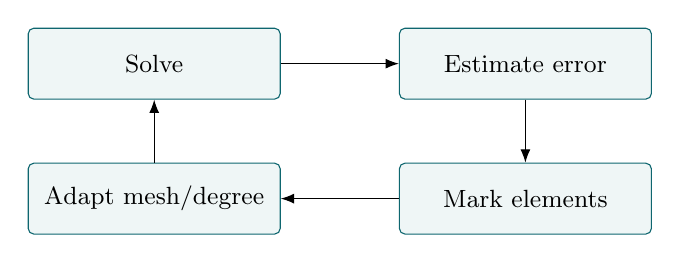
\begin{tikzpicture}[node distance=8mm and 15mm,>=Latex,
box/.style={draw=accent,rounded corners=2pt,fill=pale,minimum width=32mm,minimum height=9mm,font=\small}]
\node[box](solve){Solve};
\node[box,right=of solve](estimate){Estimate error};
\node[box,below=of estimate](mark){Mark elements};
\node[box,left=of mark](refine){Adapt mesh/degree};
\draw[->](solve)--(estimate);
\draw[->](estimate)--(mark);
\draw[->](mark)--(refine);
\draw[->](refine)--(solve);
\end{tikzpicture}
\end{center}
Bulk or Dorfler marking chooses a set $\mathcal M$ such that
\begin{equation}
\sum_{K\in\mathcal M}\eta_K^2\ge\theta\sum_K\eta_K^2,
\qquad 0<\theta<1.
\end{equation}
It controls a fraction of estimated error, unlike selecting a fixed fraction of elements irrespective of their contributions.

The axioms-of-adaptivity framework establishes convergence and quasi-optimal rates for schemes satisfying estimator stability, estimator reduction, quasi-orthogonality, and discrete reliability, with appropriate marking and refinement assumptions. These results do not automatically cover arbitrary remeshing, anisotropic aspect ratios, nonlinear shock sensors, or all transient equations~\cite{axioms}.

\heuristic Start with isotropic local refinement and a residual estimator for coercive diffusion. Keep a uniform-refinement baseline. Log error versus degrees of freedom and wall time, including the cost of estimation and remeshing. Choose marking parameters by measured tradeoffs rather than treating one value as theoretically optimal everywhere.

\subsection{Goal-oriented adaptation: refine for the answer you need}
Let $J(u)$ be an average, integrated flux, sensor response, or another output. For a linear variational problem, define the adjoint by
\begin{equation}
a(w,z)=J(w)\quad\text{for all admissible }w.
\end{equation}
With residual $\mathcal R(u_h)(v)=\ell(v)-a(u_h,v)$,
\begin{equation}\label{eq:dwr}
J(u)-J(u_h)=\mathcal R(u_h)(z)
=\mathcal R(u_h)(z-z_h)
\end{equation}
for any $z_h$ in the Galerkin test space. This identity explains why the adjoint weights the regions whose errors affect the output~\cite{becker}.

Computing $z_h$ in exactly the same space and using it directly gives zero residual by orthogonality. Practical DWR therefore needs enrichment, reconstruction, or another nontrivial adjoint approximation. For nonlinear problems, linearization and remainder terms enter. Transient outputs generally require a backward-in-time adjoint and access to the forward trajectory.

An output may be accurately predicted while the field remains inaccurate elsewhere. Singular point evaluations and derivative outputs need special care because they may not be bounded functionals on the chosen space. Stabilization also has to be reflected consistently in adjoint/error analysis.

\decision{Offer separate objectives: field accuracy in a stated norm, or accuracy in a named output. They justify different refinement decisions. Do not interpret a stable output over two meshes as a rigorous error bound.}

\section{Directional refinement and anisotropic meshes}\label{sec:anisotropy}
\subsection{Solution curvature gives directions, not just a size}
Let $H(u)=Q\operatorname{diag}(\lambda_1,\lambda_2)Q^T$. A local Taylor argument shows that linear interpolation error along a direction $q_i$ scales like $\abs{\lambda_i}h_i^2$. Under an elementwise error budget $\varepsilon_{\rm int}$, a conceptual sizing rule is
\begin{equation}\label{eq:metric}
h_i\propto\sqrt{\frac{\varepsilon_{\rm int}}
{\max(\abs{\lambda_i},\lambda_{\rm floor})}},\qquad
M=Q\operatorname{diag}(h_1^{-2},h_2^{-2})Q^T.
\end{equation}
Elements should have roughly unit edge lengths in this metric: $e^TMe\approx1$. Large curvature means shorter edges in that direction. This is an explanatory local interpolation rule, not a universal globally optimal metric. The selected norm, degree, complexity budget, and PDE weights alter metric formulas~\cite{freefem}.

For a field varying across a thin front and little along it, elements can be thin normal to the front and long tangentially. Flow direction is not always the direction needing finest resolution: a shear or crosswind layer may vary fastest perpendicular to flow.

Since the elementwise Hessian of affine $P_1$ functions is zero, recover a Hessian from neighboring values, gradients, or an enriched error estimate. Limit metric eigenvalues, aspect ratios, and spatial gradation; maintain boundary and interface constraints. With several fields, combine normalized error requirements rather than allowing a field with larger units to dominate.

\subsection{Coefficient anisotropy and solution anisotropy are distinct}
Eigenvectors of $D$ describe directional operator stiffness. Eigenvectors of $H(u)$ describe local solution curvature. They need not coincide. Sources and boundary data can rotate or eliminate solution features even when $D$ is constant. An effective metric may combine both, depending on whether the objective is interpolation accuracy, an energy norm, or preservation of a maximum principle.

For $P_1$ diffusion, nonobtuse angles in an appropriate diffusion-dependent metric provide a sufficient route to a discrete maximum principle under the paper's hypotheses. Li and Huang develop such conditions and adaptive metrics. Accuracy-oriented meshes can violate these conditions, so a small energy error and absence of negative concentrations are different achievements~\cite{lihuang}.

An elongated element is not automatically bad. It can efficiently approximate an elongated feature. But standard isotropic error estimates assume shape regularity; indiscriminately stretching elements can invalidate those bounds, worsen conditioning, and complicate multigrid. Directional refinement must be matched to an anisotropic analysis and solver strategy.

\subsection{\texorpdfstring{$h$, $p$, $hp$}{h, p, hp}, and node movement}
\begin{itemize}
\item $h$ adaptation changes element sizes. It is effective near singularities and localized nonsmooth behavior.
\item $p$ adaptation increases local degree. Smooth or analytic fields can benefit strongly, but unresolved layers and geometric error may prevent that benefit.
\item $hp$ adaptation combines geometric grading near singularities with increased degree in smooth regions. Exponential convergence is proved for specified regularity and mesh constructions, not for any automatic $h/p$ switch~\cite{hp}.
\item $r$ adaptation moves nodes with fixed connectivity. It can track fronts, but needs mesh-quality control and correct moving-mesh equations or conservative remapping.
\end{itemize}
Smoothness decisions can use modal coefficient decay, enriched solutions, or estimated error reductions per additional degree of freedom. These are algorithmic indicators with model-dependent reliability. Hanging nodes or nonmatching refinements require constraints or compatible interface treatment.

\decision{Learn isotropic adaptation before implementing anisotropic remeshing. Then compare Hessian-based sizing with an error-based directional strategy. Measure solver iterations and explicit time-step penalties as well as approximation error.}

\section{Time integration must match the semidiscrete spectrum}\label{sec:time}
\subsection{Method of lines retains a mass matrix}
Spatial FEM yields, for a linear problem,
\begin{equation}\label{eq:mol}
M_2\ddot U+M_1\dot U+AU=F(t).
\end{equation}
For first-order evolution, $M_1\dot U+AU=F$. If $M_1$ is invertible, the evolution operator is $L=-M_1^{-1}A$. Do not form a dense inverse. Apply a mass solve, use an appropriate lumped mass, or use an integrator accepting an implicit residual.

For second-order evolution, set $V=\dot U$:
\begin{equation}
\begin{pmatrix}I&0\\0&M_2\end{pmatrix}
\begin{pmatrix}\dot U\\\dot V\end{pmatrix}
=\begin{pmatrix}V\\F-AU-M_1V\end{pmatrix}.
\end{equation}
This reduces temporal order if $M_2$ is invertible. If some variables have no time derivative or impose constraints, the system can instead be a DAE. Compatible initial data and a suitable DAE formulation are required~\cite{petscts}.

\subsection{Diffusion: stability and damping}
For a diffusion eigenmode with $A\phi=\lambda M\phi$, $\lambda\ge0$, the amplitude satisfies $y'=-\lambda y$. Forward Euler gives amplification $1-\Delta t\lambda$, so
\begin{equation}
\Delta t\le\frac{2}{\lambda_{\max}(M^{-1}A)}.
\end{equation}
On standard low-order meshes the maximum eigenvalue scales like $d/(\rho_1h_{\min}^2)$, with mesh and coefficient factors. Refining a small region can limit the global step. On anisotropic meshes, the shortest relevant directional scale can dominate; a single average $h$ is misleading.

Backward Euler has amplification $(1+\Delta t\lambda)^{-1}$ and strongly damps stiff modes. Crank--Nicolson has amplification
\begin{equation}
g_{\rm CN}=\frac{1-\Delta t\lambda/2}{1+\Delta t\lambda/2}.
\end{equation}
As $\Delta t\lambda\to\infty$, this tends to $-1$: it is stable but can preserve alternating high-frequency numerical transients. Large stable time steps can still be inaccurate. Implicit stability is not permission to skip temporal convergence studies.

BDF methods and implicit Runge--Kutta schemes offer other order/stability tradeoffs. Variable-order BDF implementations control local errors and nonlinear solves; tolerances weight variables by absolute and relative scales~\cite{sundials}. Nonlinear iteration failure, discontinuous forcing, and remeshing can affect step acceptance.

\subsection{Waves: phase accuracy and energy}
For $M\ddot U+KU=0$ with symmetric positive $M,K$, the semidiscrete energy
\begin{equation}
E_h=\tfrac12\dot U^TM\dot U+\tfrac12U^TKU
\end{equation}
is constant because $\dot E_h=\dot U^T(M\ddot U+KU)=0$. Damping, boundary work, or forcing changes this balance predictably.

For central differences on a mode $y''+\omega_h^2y=0$, stability requires $\Delta t\omega_h\le2$. Thus $\Delta t\le2/\sqrt{\lambda_{\max}(M^{-1}K)}$. This is not the forward-Euler diffusion restriction. Forward Euler on the first-order oscillator has eigenvalues $\pm i\omega_h$ and amplifies them for every nonzero step.

The central-difference dispersion relation is
\begin{equation}
\omega_{\rm num}=\frac{2}{\Delta t}
\arcsin\left(\frac{\omega_h\Delta t}{2}\right).
\end{equation}
Even a stable step has phase error. Spatial FEM already perturbs $\omega_h$, so spatial and temporal dispersion must be assessed together. Implicit midpoint conserves this linear quadratic energy, but still has frequency error; generalized-alpha methods deliberately control high-frequency damping. Energy conservation alone does not certify an accurate wave trajectory.

\subsection{Advection, IMEX, and splitting}
Explicit transport restrictions scale like $\Delta t B/(\rho_1h_\parallel)\lesssim C$, with $C$ depending on the spatial formulation, degree, and integrator. Pure imaginary spectra are unsuitable for forward Euler; nonnormal operators can exhibit growth not predicted by eigenvalues alone. Assess an energy bound or amplification operator when necessary.

IMEX treats a stiff part implicitly and another part explicitly. It can avoid a diffusive $h^2$ restriction while retaining a transport restriction, but the split must be deliberate and its coupling behavior checked~\cite{petscts}. Lie splitting is generally first-order; Strang splitting is second-order under suitable smoothness and compatibility, with possible order reduction from stiff terms or boundaries. Cheap subsolves do not remove splitting error.

\subsection{Adapt space and time together}
Balance estimated spatial, temporal, algebraic, and transfer errors. Embedded time estimates control the error of the semidiscrete trajectory, not the error caused by an underresolved spatial field. Conversely, refining space on every tiny time step can be wasteful.

Changing meshes requires transfer of state. Interpolation can alter mass and energy. An $L^2$ projection with constants represented preserves the global integral under exact integration on the same domain, but does not automatically preserve positivity or local balance. Wave transfer involves both displacement and velocity; BDF also involves time history. Moving coordinates require the associated mesh-velocity terms.

\decision{Implement one verified diffusion integrator and one verified wave integrator before a large menu. Log the limiting stability scale, accepted step sizes, temporal tolerances, and physical balance defects.}

\section{Linear solvers: use the assembled operator's structure}\label{sec:solvers}
\subsection{Choose a solver and a preconditioner together}
The algebraic operator may be a stiffness matrix, $M+\Delta t A$, or a Newton Jacobian. Its properties depend on constraints, stabilization, and time step as well as the original PDE. PETSc explicitly separates Krylov iteration from preconditioning and supports both assembled and operator-based systems~\cite{petscksp}.

\begin{longtable}{P{0.23\textwidth}P{0.27\textwidth}P{0.42\textwidth}}
\toprule
Matrix property & Candidate solve & Qualification\\
\midrule\endhead
Real symmetric positive definite & Cholesky or CG & Standard preconditioned CG requires a compatible SPD preconditioner. Symmetric PDE coefficients alone do not guarantee the final matrix is SPD.\\
Real symmetric indefinite & Sparse LDL$^T$ or MINRES & MINRES also requires symmetry and a suitable SPD preconditioner in the standard setting.\\
Nonsymmetric & Sparse LU, GMRES; possibly BiCGStab & GMRES memory grows with Krylov basis size; restart can impair convergence. BiCGStab is cheaper in storage but can be less predictable.\\
Variable/nonlinear preconditioning & FGMRES & Useful when an inner solve or preconditioner changes during iterations.\\
Saddle point or multiphysics blocks & Block Krylov with Schur or field-split preconditioning & Preserve field structure and supply an appropriate approximation for each block.\\
Singular compatible system & Nullspace-aware solve or constrained solve & Check right-hand-side compatibility and define which representative solution is required.\\
\bottomrule
\end{longtable}

Direct sparse factorization is valuable for small two-dimensional reference problems, debugging, and many right-hand sides. Its fill and memory can grow substantially, especially in three dimensions. Iterative solvers become attractive when preconditioning keeps iteration counts controlled. The crossover is empirical and problem-dependent~\cite{elman}.

\subsection{Multigrid and PDE-informed preconditioning}
Multigrid combines a smoother for oscillatory error with a coarse correction for error poorly reduced by that smoother. Geometric multigrid uses a mesh/space hierarchy. AMG builds a hierarchy from algebraic couplings and can use supplied near-nullspace information.

Coefficient contrast, anisotropy, stretched cells, and constraints change what error is difficult. Point smoothing may fail to reduce error associated with strong directional coupling; line/block smoothing, semi-coarsening, suitable strength-of-connection rules, or more robust coarse spaces can help. The hypre documentation exposes different coarsening, interpolation, and smoothing options, including block, Schwarz, and ILU smoothers~\cite{hypre}.

Ordinary diffusion-oriented AMG is not automatically robust for high-frequency indefinite Helmholtz operators. Shifted-Laplacian, sweeping/domain-decomposition, and wave-aware coarse-space approaches are separate research areas. A method that works well at low frequency may stagnate at high frequency.

For a coupled matrix
\begin{equation}
\mathcal A=\begin{pmatrix}A&B\\C&D\end{pmatrix},\qquad
S=D-CA^{-1}B,
\end{equation}
block elimination suggests a Schur-complement preconditioner. Approximate actions of $A^{-1}$ and $S^{-1}$ are used; dense inverses need not be formed. PDE structure suggests whether a mass matrix, pressure Laplacian, or another operator approximates $S$. A poor Schur approximation can negate the value of excellent individual field solvers~\cite{petscfield}.

\subsection{Stopping criteria are part of the numerical method}
A small algebraic residual does not imply a small PDE error. For an SPD system, if $e_A=U-U_* $ and $r=b-AU$, then $\norm{e_A}_A^2=r^TA^{-1}r$. A reliable preconditioner can make a residual-based energy estimate useful. A raw relative residual without scaling or conditioning information is not a universal error measure.

\heuristic On coarse meshes solve tightly enough to diagnose assembly. For production studies, keep algebraic error demonstrably below the dominant discretization error, then stop. A fixed value such as $10^{-12}$ for every mesh may waste substantial work. Monitor convergence reasons, true residuals, iteration counts, setup cost, and memory; a returned vector is not proof of convergence.

\decision{Select from documented mathematical properties, then check the actual constrained operator. Reuse factorizations only when the matrix is unchanged. Reusing a preconditioner after coefficient, mesh, or time-step changes is a measured tradeoff.}

\section{Nonlinear PDEs and coupled processes}\label{sec:nonlinear}
\subsection{The Jacobian can differ qualitatively from the original operator}
For a nonlinear residual $\mathcal F(U)=0$, Newton solves
\begin{equation}
J(U_k)\delta U=-\mathcal F(U_k),\qquad
U_{k+1}=U_k+\alpha_k\delta U.
\end{equation}
For nonlinear diffusion, varying $\int D(u)\nabla u\cdot\nabla v$ gives
\begin{equation}
\int D(u)\nabla\delta u\cdot\nabla v
+\int D'(u)\delta u\,\nabla u\cdot\nabla v.
\end{equation}
The second term can destroy symmetry. ``Diffusion equation, therefore CG'' is then wrong. By contrast, a monotone semilinear reaction $-\Delta u+g(u)=f$ with $g'(u)\ge0$ gives a symmetric positive Jacobian with suitable Dirichlet conditions.

Newton has fast local convergence under standard differentiability and nonsingularity assumptions, not global convergence from arbitrary initial states. Line search, trust region, parameter continuation, and admissibility checks improve robustness. Picard iteration can be easier to formulate and precondition but is not guaranteed to converge either~\cite{petscsnes}.

Inexact Newton allows looser linear solves when far from the solution and tightens them as needed. Differentiate a residual consistently, including constitutive and stabilization terms unless a justified approximation is intended. Verify Jacobian actions against directional finite differences. Nonsmooth laws may require semismooth or specialized solvers.

\subsection{Multiphysics is a coupled numerical problem}
For two processes, a monolithic solve includes the off-diagonal couplings in one residual/Jacobian. A segregated solve alternates subproblems. It can be economical for weak coupling, while strong feedback may converge slowly or become unstable unless iteration, relaxation, or a better splitting is used.

Time-scale separation can justify quasistatic treatment of one field; it must come from physical scaling and error assessment. It is not justified solely because the elliptic subproblem is easier to solve. A charge/field/transport simulation can change its own coefficients and refine regions as the state evolves.

\decision{Add nonlinear scalar diffusion or reaction only after linear adaptation and time integration work. Study one controlled coupling before treating arbitrary systems as an extension of scalar assembly.}

\section{Other choices that strongly affect efficiency}\label{sec:performance}
\subsection{Quadrature, geometry maps, and coefficient evaluation}
With degree-$p$ affine elements and constant coefficients, diffusion integrands have degree $2p-2$ and mass integrands degree $2p$. Variable coefficients and curved maps change this; nonlinear terms may require overintegration. Underintegration can introduce rank defects, aliasing, or inaccurate residuals. More quadrature does not repair incorrect interface integration.

Element maps transform gradients by $J_K^{-T}$ and integration weights by $\abs{\det J_K}$. Check positive orientation, nonsingular maps, normals, and correct tensor transformation. For curved elements, sampling a Jacobian at too few points may miss inversion between samples.

Cache reference basis values and quadrature data. Reuse sparsity patterns on a fixed mesh, constant geometry factors where appropriate, and time-independent matrices. Changing degree, constraints, topology, or nonlinear coefficients changes what may be reused. These are direct consequences of the weak form rather than universal cache rules.

\subsection{Assembly versus operator application}
For suitable tensor-product high-order elements, the operator can be expressed schematically as
\begin{equation}
A=P^TG^TB^TDBG P,
\end{equation}
where $P$ handles global constraints/parallel distribution, $G$ element restriction, $B$ basis evaluation, and $D$ quadrature-point physics. Full assembly stores a sparse matrix; partial assembly stores selected factors; matrix-free evaluation applies the operator without storing the full matrix~\cite{mfem}.

With $n\sim p$ points per coordinate in $d$ dimensions, dense local application costs roughly $O(n^{2d})$. Tensor sum factorization reduces basis application to approximately $O(dn^{d+1})$. This estimate concerns suitable tensor-product kernels, not every triangular discretization or the entire solve.

Matrix-free multiplication can be fast while total solve time is poor if the preconditioner is weak. Low-order assembled approximations, $p$-multigrid, or geometric multigrid can supply preconditioning. GPU speedups depend on batch size, degree, memory movement, and synchronization; a small learning problem may not amortize them~\cite{ceed}.

\subsection{Conservation, positivity, dispersion, and entropy}
Accuracy in one norm does not ensure every physical property. Track global mass balance, cellwise flux balance when required, maximum-principle violations when applicable, and wave energy/phase. For nonlinear hyperbolic limits, entropy admissibility can select the physically relevant weak solution. Conservative fluxes and appropriate limiters are essential tools; high order alone is insufficient~\cite{leveque}.

Continuous Galerkin can preserve a global balance under suitable tests and boundary treatment, yet its raw reconstructed flux need not conserve elementwise. Mass lumping changes the discrete model, dispersion, and sometimes monotonicity. It is not merely an implementation shortcut.

\subsection{Conditioning is not sensitivity of the physical model}
Nondimensionalize and scale unknowns, equations, and tolerances. Mesh refinement increases algebraic condition numbers even when the continuous problem is well posed. Physical resonance or nearly degenerate coefficients can also amplify input uncertainty. These mechanisms should be diagnosed separately. A numerical error certificate does not remove uncertainty in material parameters, boundary data, or the modeling assumptions.

\section{What published experiments show, and what they do not}\label{sec:empirical}
\subsection{Directional error information changes the result}
\evidence Huang, Kamenski, and Lang compare anisotropic strategies for a manufactured Poisson field containing steep fronts. Their Figure~3 reports the following meshes and true $L^2$ errors~\cite{huangkamenski}:
\begin{center}
\begin{tabular}{lrrr}
\toprule
Estimator driving the metric & Triangles & $L^2$ error & Max. aspect ratio\\
\midrule
Edge-based local & 1,345 & $5.0\times10^{-3}$ & 12.8\\
Node-based local & 1,339 & $3.7\times10^{-3}$ & 14.3\\
Full hierarchical & 1,413 & $1.6\times10^{-3}$ & 46.9\\
\bottomrule
\end{tabular}
\end{center}
The meshes have comparable, not identical, counts. Better orientation accompanies substantially lower error in this example. The authors also report that three symmetric Gauss--Seidel steps for the auxiliary error problem produced nearly the same adaptation quality as a much more accurate solve. This does not establish a universal iteration count. The work was published in 2010; the arXiv copy was uploaded in 2019.

\textbf{Inference for your project.} A scalar error magnitude can tell you where to refine while missing how to orient elements. Auxiliary estimates should be accurate enough to make decisions; oversolving them may have little benefit.

\subsection{A good-looking diffusion solution can violate a maximum principle}
\evidence Li and Huang study anisotropic $P_1$ diffusion with metrics designed for accuracy, maximum-principle compliance, or both. In Example~5.1 the diffusion eigenvalues are $1000$ and $1$, and the exact field is constrained between boundary values $0$ and $2$. Their accuracy-oriented and near-uniform meshes can produce undershoots, while the meshes satisfying the derived sufficient DMP conditions remove these violations. They also discuss an accuracy cost for DMP constraints~\cite{lihuang}.

\textbf{Inference.} Report error and admissibility separately. A mesh optimized for one criterion does not automatically optimize the other.

\subsection{Removing oscillations is not the same as resolving a layer}
\evidence John and Knobloch compare stabilization methods on stationary two-dimensional convection-diffusion tests with $\varepsilon=10^{-8}$, including boundary and interior layers. They report substantial improvements over SUPG in some cases, but also cases where suppressed oscillations coexist with smearing or an incorrect field in a region expected to vanish. Their comparison measures both oscillation and layer-smearing behavior~\cite{johnknobloch}.

\textbf{Inference.} A stabilization parameter should not be accepted because the plot becomes smooth. Their findings concern the formulations and tests examined; they are not a claim that all later bound-preserving methods fail.

\subsection{High-order performance depends on architecture and problem size}
\evidence The CEED study reports throughput/latency comparisons for high-order Poisson benchmark BP3 on CPU and GPU hardware. In its reported CPU/V100 comparison, small GPU kernels are dominated by overhead, while larger batches obtain substantially better throughput. It also demonstrates that kernel fusion changes performance~\cite{ceed}.

\textbf{Inference.} Benchmark complete solves at equal accuracy on your target hardware. An operator-kernel throughput comparison is not a promise of faster small two-dimensional solves, and a benchmark on older hardware does not set a universal current crossover.

\subsection{An original reproducible FEM experiment}
Solve
\begin{equation}\label{eq:experiment}
-0.01u''+u'=0,\qquad x\in(0,1),\qquad u(0)=0,\quad u(1)=1.
\end{equation}
The exact solution is
\begin{equation}
u(x)=\frac{\exp((x-1)/0.01)-\exp(-100)}{1-\exp(-100)}.
\end{equation}
Use uniform continuous $P_1$ FEM with exact local matrix integration and strong endpoint elimination. Compare Galerkin, SUPG with~\eqref{eq:tau}, and an upwind-equivalent artificial diffusion $d_{\rm eff}=d+Bh/2$. Compute the true error of the piecewise-linear field using 32-point Gauss--Legendre quadrature per element. These numbers were computed for this guide; they are not a published two-dimensional benchmark.

\begin{center}
\small
\begin{tabular}{rrlrr}
\toprule
Elements & $\mathrm{Pe}_h$ & Method & $\min u_h$ & $\norm{u-u_h}_{L^2}$\\
\midrule
10 & 5.000 & Galerkin & $-0.696079$ & $0.191479$\\
10 & 5.000 & SUPG & $0$ & $0.142600$\\
10 & 5.000 & Upwind-equivalent & $0$ & $0.154151$\\
20 & 2.500 & Galerkin & $-0.428571$ & $0.077949$\\
20 & 2.500 & SUPG & $0$ & $0.075677$\\
20 & 2.500 & Upwind-equivalent & $0$ & $0.093759$\\
40 & 1.250 & Galerkin & $-0.111111$ & $0.026262$\\
40 & 1.250 & SUPG & $0$ & $0.030354$\\
40 & 1.250 & Upwind-equivalent & $0$ & $0.052712$\\
80 & 0.625 & Galerkin & $0$ & $0.007364$\\
80 & 0.625 & SUPG & $0$ & $0.009274$\\
80 & 0.625 & Upwind-equivalent & $0$ & $0.028165$\\
\bottomrule
\end{tabular}
\end{center}

\begin{figure}[htbp]
\centering
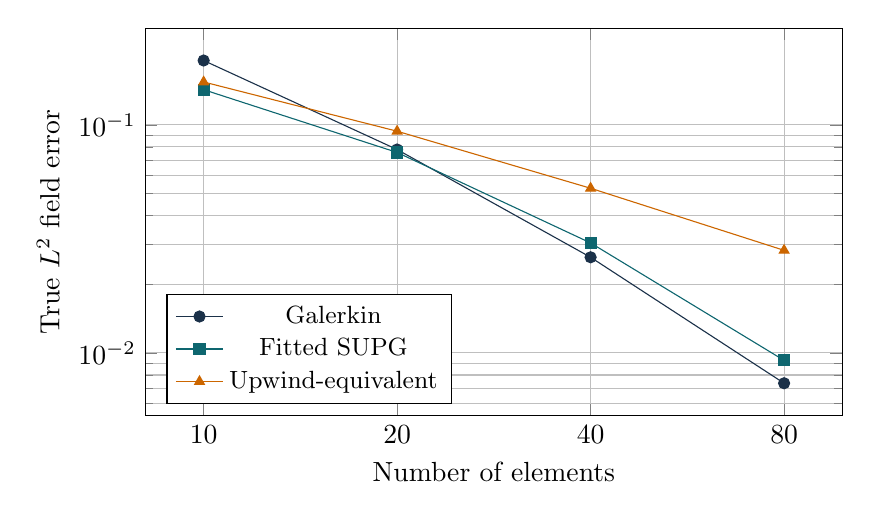
\begin{tikzpicture}
\begin{loglogaxis}[width=0.86\textwidth,height=65mm,
xlabel={Number of elements},ylabel={True $L^2$ field error},
grid=both,legend pos=south west,legend style={font=\small},
xtick={10,20,40,80},xticklabels={10,20,40,80}]
\addplot[color=ink,mark=*] coordinates {(10,0.191479)(20,0.077949)(40,0.026262)(80,0.007364)};
\addlegendentry{Galerkin}
\addplot[color=accent,mark=square*] coordinates {(10,0.142600)(20,0.075677)(40,0.030354)(80,0.009274)};
\addlegendentry{Fitted SUPG}
\addplot[color=orange!80!black,mark=triangle*] coordinates {(10,0.154151)(20,0.093759)(40,0.052712)(80,0.028165)};
\addlegendentry{Upwind-equivalent}
\end{loglogaxis}
\end{tikzpicture}
\caption{Original one-dimensional $P_1$ experiment. Removing negative values does not guarantee the lowest $L^2$ field error. The plot is an accuracy comparison, not a runtime benchmark.}
\end{figure}

\textbf{What this isolates.} Galerkin violates the maximum principle on the three coarse meshes. Fitted SUPG gives nodally exact values in this special constant-coefficient one-dimensional setting, but the piecewise-linear field still has interpolation error inside elements. At 40 elements, Galerkin has lower $L^2$ error despite a negative minimum. At 80 elements, it is monotone and has lower field error than both stabilized choices. Thus ``most stable,'' ``nodally exact,'' and ``smallest field error'' are different statements.

This experiment does not establish a universal SUPG ranking or Peclet threshold for arbitrary meshes. Appendix~\ref{app:stencil} gives the matrix entries needed to reproduce it without a specialized PDE package.

\section{Worked decisions for your geometry-based engine}\label{sec:cases}
\subsection{Case A: smooth diffusion on a rectangle or circle}
\textbf{Input.} $-\nabla\cdot(D\nabla u)+\sigma u=f$, symmetric uniformly positive $D$, $\sigma\ge0$, suitable Dirichlet or Robin data.

\textbf{Analysis.} Prove coercivity from coefficient signs and boundary constraints. Estimate coefficient contrast; identify any known interfaces. A circle additionally requires a geometry-accuracy decision.

\textbf{First method.} Continuous $P_1$, adequate quadrature, symmetric constraint elimination, sparse direct reference solve. Then compare CG with multilevel preconditioning. Measure $H^1$ and $L^2$ convergence using a manufactured solution, including curved-boundary effects.

\textbf{Improvement.} Use a residual adaptive loop if error is localized. Compare $P_2$ with refined $P_1$ for smooth fields. Keep the same error target and include setup cost. If flux conservation matters, compare a reconstructed equilibrated flux or mixed method.

\subsection{Case B: rotated anisotropic diffusion with a narrow source}
\textbf{Input.} $D=Q\operatorname{diag}(1,10^{-3})Q^T$ for a rotated $Q$, plus a localized smooth source.

\textbf{Analysis.} The operator remains elliptic, but directions and length scales differ greatly. Source width must be resolved independently of a pilot solution. Tensor eigenvectors predict possible behavior; they do not determine the optimal mesh alone.

\textbf{First method.} A sufficiently resolved isotropic mesh, $P_1$ Galerkin, and a direct solve to isolate approximation error from iterative failure.

\textbf{Improvement.} Compare isotropic residual refinement, a recovered-curvature metric, and a coefficient-aware metric. Repeat at several tensor rotations and source locations. Evaluate energy error, minima/maxima if relevant, metric quality, solve iterations, and wall time. If AMG degrades, investigate its coarse space and smoother before concluding that directional meshes are ineffective.

\subsection{Case C: convection-diffusion with an outflow layer}
\textbf{Input.} $u_t-\varepsilon\Delta u+\beta\cdot\nabla u=f$ with small positive $\varepsilon$ and prescribed boundary data.

\textbf{Analysis.} Compute element Peclet diagnostics and inflow/outflow regions. Balance transport and diffusion to estimate layer scales. The equation is still parabolic for positive diffusion; this label does not justify unstabilized Galerkin on a coarse mesh.

\textbf{First method.} Test standard Galerkin as a baseline and SUPG as a supported transport method. Keep the layer resolution and time discretization explicit in the experiment.

\textbf{Improvement.} Adapt normal to the layer; assess positivity, smearing, and output flux. Compare an implicit diffusion/explicit transport split only after checking the transport stability region. At $\varepsilon=0$, switch to a verified transport formulation and inflow boundary policy instead of reusing the diffusion problem unchanged.

\subsection{Case D: wave propagation or time-harmonic Helmholtz}
\textbf{Input.} $u_{tt}-c^2\Delta u=f$ or $-\Delta u-k^2u=f$.

\textbf{Analysis.} Transient waves require two initial conditions and compatible boundary data. Harmonic Helmholtz requires analysis of resonance and radiation conditions. Wavelength resolution is necessary, but phase error accumulates with distance and frequency. Wavenumber-explicit Helmholtz analysis shows that mesh/degree conditions depend on stability and regularity, not simply a fixed points-per-wavelength rule~\cite{melenk}.

\textbf{First method.} For transient waves, $P_1$ with a verified mass treatment and central differences or implicit midpoint; monitor phase and energy. For Helmholtz, use sparse LU as a small-problem reference. The matrix can be indefinite even though the spatial principal operator is elliptic.

\textbf{Improvement.} Compare higher degree and refined meshes at equal phase accuracy over the intended travel distance. Separate boundary reflection error from discretization dispersion. Absorbing conditions and PML introduce modeling/truncation and discretization parameters of their own; test thickness, absorption, and mesh resolution independently.

\section{Verification, error budgets, and fair comparisons}\label{sec:verification}
\subsection{Separate the errors before optimizing}
A conceptual budget is
\begin{equation}
E_{\rm total}\lesssim E_{\rm model}+E_{\rm geometry}+E_{\rm space}
+E_{\rm time}+E_{\rm quadrature}+E_{\rm algebra}+E_{\rm transfer}.
\end{equation}
The terms need compatible norms or output measures, and in many settings this is an organizational decomposition rather than a rigorous additive bound. It is still useful: driving algebraic error to machine precision while geometry dominates cannot improve the answer.

\subsection{Manufactured solutions and invariants}
Choose a smooth $u_\star(x,y,t)$, substitute it into the intended PDE to generate $f$, and derive boundary and initial data from the same function. For example,
\begin{equation}
u_\star=e^{-t}\sin(\pi x)\sin(\pi y),\qquad
u_t-\Delta u=(2\pi^2-1)u_\star
\end{equation}
on the unit square with zero Dirichlet data. Rotated variable tensors and nonzero mixed boundary conditions expose more code paths. NASA's LAVA verification work illustrates MMS alongside benchmark and experimental validation in an engineering solver workflow~\cite{nasa}.

Compute observed order $q=\log(E_h/E_{h/2})/\log2$ only when the refinement ratio and asymptotic regime justify it. Tighten time and algebraic errors during a spatial study; tighten space and algebraic errors during a temporal study. On adapted meshes, plot error against degrees of freedom and actual cost rather than assigning one representative $h$.

Also test the balances implied by the model: conserved mass for suitable no-flux diffusion, decay of diffusion energy, constant undamped wave energy, known boundary work, and steady flux balance. Invariants can expose errors missed by one manufactured solution. They cannot replace convergence studies or validation against physical data.

\subsection{Experiments that teach more than a single successful run}
\begin{longtable}{P{0.23\textwidth}P{0.32\textwidth}P{0.37\textwidth}}
\toprule
Question & Controlled comparison & Record\\
\midrule\endhead
Does adaptation help? & Uniform versus residual refinement & True/estimated errors, unknowns, estimation/remeshing time.\\
Does direction matter? & Same source, rotated $D$ and mesh & Energy error, orientation, aspect ratios, iteration counts.\\
Is stabilization accurate? & Galerkin/SUPG/another verified scheme across Peclet regimes & Minimum/maximum, layer width, field error, flux balance.\\
Is higher degree cheaper? & $P_1$ refinement versus $P_2$ or $hp$ & Total time and memory at matched error.\\
Is the transient solution correct? & Independent space and step refinement & Phase, amplitude, energy/balance, temporal order.\\
Does the solver scale? & Direct versus Krylov/preconditioner across meshes & Setup/apply/solve time, residual reason, memory.\\
Does the estimator track error? & Known-solution tests and difficult interfaces & Effectivity $\eta/E$, localization, sensitivity to contrast.\\
\bottomrule
\end{longtable}
Use several cases per regime and include failure cases. A solver configured for one benchmark can win that benchmark while becoming unreliable when coefficient orientation, boundary data, or degree changes. Hold accuracy and physical admissibility requirements fixed when comparing speed.

\section{A practical study and implementation sequence}\label{sec:roadmap}
\subsection{Stage 1: make one mathematical contract reliable}
Support fixed two-dimensional domains, scalar divergence-form diffusion, symmetric positive tensor coefficients, continuous $P_1$ triangles, and labeled Dirichlet/Neumann/Robin data. Include coefficient interfaces and pure-Neumann compatibility/nullspace treatment deliberately. Use a direct reference solver.

\textbf{Learn:} coercivity, weak forms, interpolation error, geometric mapping, quadrature, constraints.\quad
\textbf{Exit criterion:} known-solution convergence and balance tests work across the supported geometries and boundary combinations.

\subsection{Stage 2: connect PDE structure to accuracy and cost}
Add residual error estimation, bulk marking, conforming refinement/constraints, and CG with a suitable preconditioner. Keep the uniform-mesh baseline. Add $P_2$ only when the baseline is established.

\textbf{Learn:} reliability versus efficiency, data oscillation, regularity, multigrid, error versus work.\quad
\textbf{Exit criterion:} adaptive meshes demonstrably improve specified cases, and algebraic error is controlled relative to discretization error.

\subsection{Stage 3: add first-order time dependence}
Assemble mass matrices and implement backward Euler and Crank--Nicolson, or another small verified set. Study a sharp initial condition to expose damping differences. Then add adaptive step control and mesh transfer if justified.

\textbf{Learn:} generalized spectra, stiffness, stability versus accuracy, mass conservation, separate space/time studies.\quad
\textbf{Exit criterion:} correct temporal order and balance under independent refinement, including changing forcing and boundaries.

\subsection{Stage 4: introduce a difficult PDE regime explicitly}
Choose convection-diffusion with SUPG \emph{or} anisotropic diffusion with metric adaptation as the next focus. Each exposes a different limitation of baseline FEM. Add both eventually, but isolate their effects during learning.

\textbf{Learn:} singular perturbations and monotonicity for transport; directional interpolation and solver robustness for anisotropy.\quad
\textbf{Exit criterion:} a documented parameter range, failure diagnostics, and measured accuracy/cost comparisons.

\subsection{Stage 5: waves, nonlinearities, and outputs}
Add second-order time evolution and dispersion/energy diagnostics. Add monotone nonlinear reaction or nonlinear diffusion with a verified Jacobian and globalization. Then implement one quantity-of-interest adjoint and goal-oriented adaptation. Mixed systems, DG, $hp$, and matrix-free/GPU kernels become focused extensions after these capabilities are understood.

\textbf{What the engine should explain for each solve.} Which mathematical family is supported; what scale and sign diagnostics were used; why the formulation, mesh policy, time method, and solver are eligible; what error or convergence evidence is available; and which assumptions remain unverified. This is numerical transparency, not a claim that software can prove all properties of arbitrary supplied functions.

\textbf{Recommended scope.} A well-tested family covering diffusion, transport-diffusion, and waves on several geometries will teach much more than an unrestricted equation input that assembles a matrix and hopes the result is meaningful.

\section{Reading map: methods first, implementations second}\label{sec:reading}
\begin{longtable}{P{0.13\textwidth}P{0.40\textwidth}P{0.39\textwidth}}
\toprule
Priority & Resource & Study purpose\\
\midrule\endhead
1 & Ern and Guermond, \emph{Theory and Practice of Finite Elements}~\cite{ernclassic}; selected parts of \emph{Finite Elements I--II}~\cite{ern1,ern2} & Function spaces, approximation, stability, consistency, mixed formulations. Use as reference rather than reading all volumes before coding.\\
2 & Elman, Silvester, Wathen, \emph{Finite Elements and Fast Iterative Solvers}, 2nd ed.~\cite{elman} & Closest match to your goal: connect PDE discretization with efficient algebraic solution.\\
3 & Bangerth and Rannacher, \emph{Adaptive Finite Element Methods for Differential Equations}~\cite{bangerth} & Residual and goal-oriented error control; understand the adaptive feedback loop.\\
4 & Roos, Stynes, Tobiska, \emph{Robust Numerical Methods for Singularly Perturbed Differential Equations}~\cite{roos} & Layers, fitted meshes, stabilized methods, parameter robustness.\\
5 & LeVeque, \emph{Finite Volume Methods for Hyperbolic Problems}~\cite{leveque} & Characteristics, conservative numerical fluxes, Riemann problems and limiters; relevant beyond FEM.\\
Focused papers & Cea/inf-sup notes; axioms of adaptivity; DWR; anisotropic adaptation; Helmholtz analysis~\cite{femconvergence,suli,axioms,becker,huangkamenski,melenk} & Read the assumptions and the numerical examples side by side. Ask which decision each result actually supports.\\
Software examples & PETSc, hypre, FreeFEM, Gmsh, MFEM~\cite{petscksp,petscts,hypre,freefem,gmsh,mfem} & See how mathematical choices appear as solver, metric, time-integration, and operator interfaces.\\
\bottomrule
\end{longtable}

\appendix
\section{Reproduce the convection-diffusion experiment}\label{app:stencil}
For an element $[x_i,x_{i+1}]$ of length $h$ with the two usual linear basis functions, the diffusion and advection matrices are
\begin{equation}
A_K=\frac{d_{\rm eff}}h
\begin{pmatrix}1&-1\\-1&1\end{pmatrix}
+\frac B2\begin{pmatrix}-1&1\\-1&1\end{pmatrix}.
\end{equation}
Assemble them, set $U_0=0$, $U_N=1$, and solve the interior tridiagonal system. For SUPG in this zero-source, constant-coefficient $P_1$ problem,
\begin{equation}
d_{\rm eff}=d+\tau B^2=\frac{Bh}{2}\coth(\mathrm{Pe}).
\end{equation}
For the upwind-equivalent comparison, $d_{\rm eff}=d+Bh/2$. Reconstruct linearly between the nodes, and integrate its squared difference from the analytical field. That last step prevents a misleading conclusion based only on nodal values.

The interior Galerkin stencil has left coefficient $-d/h-B/2$, diagonal $2d/h$, and right coefficient $-d/h+B/2$. When $Bh/(2d)>1$, the right off-diagonal is positive, losing the usual M-matrix sign pattern. In this uniform one-dimensional setup, the threshold explains the oscillation behavior. It is not a universal monotonicity criterion for multidimensional FEM, variable coefficients, or transient mass matrices.

For a reproducibility check, repeat the error integration with 64 quadrature points; the rounded table entries should remain unchanged. No timing or hardware-performance conclusion is drawn from these small dense reference solves.

\section{A minimal analysis record for a supported equation}
\begin{tabularx}{\textwidth}{P{0.30\textwidth}Y}
\toprule
Item & Information that makes numerical decisions meaningful\\
\midrule
Operator & Divergence/non-divergence; temporal order; scalar/system; linear/nonlinear.\\
Coefficient bounds & Symmetry, ellipticity, contrast, anisotropy, degeneracy; analytic bounds versus sampled diagnostics.\\
Data and geometry & Boundary labels; initial data; material interfaces; singular sources; curvature; corner angles.\\
Physical structure & Conserved quantities; positivity bounds; energy or entropy; incoming characteristics.\\
Scales & Layer width; local Peclet; reaction/diffusion times; wavelength; stiffness.\\
Accuracy objective & Norm or output; spatial/temporal tolerance; geometry and transfer requirements.\\
Eligible methods & Space, stabilization, mesh policy, time integrator, algebraic solver/preconditioner.\\
Evidence & Convergence history; estimator assumptions; balances; true residual; runtime and memory.\\
\bottomrule
\end{tabularx}

\clearpage
\begin{thebibliography}{99}
\small\raggedright
\bibitem{mude} TU Delft MUDE teaching team. \emph{Introduction to PDEs}. MUDE textbook, 2025 edition. Principal-part classification and limitations of two-variable formulas.\newline\url{https://mude.citg.tudelft.nl/book/2025/numerical_methods_for_PDEs/intro_to_pdes.html}
\bibitem{femstability} Imperial College finite element course. \emph{Finite element problems: solvability and stability}. Coercivity, Lax--Milgram, nullspaces.\newline\url{https://finite-element.github.io/L4_feprobs.html}
\bibitem{femconvergence} Imperial College finite element course. \emph{Convergence of finite element approximations}. Sobolev spaces, Galerkin approximation, and error analysis.\newline\url{https://finite-element.github.io/L5_convergence.html}
\bibitem{femstokes} Imperial College finite element course. \emph{Stokes equation}. Mixed formulation and discrete stability.\newline\url{https://finite-element.github.io/L6_stokes.html}
\bibitem{suli} E. Suli. \emph{A brief excursion into the mathematical theory of mixed finite element methods}. University of Oxford lecture notes.\newline\url{https://people.maths.ox.ac.uk/suli/mixed_FEM_lectures.pdf}
\bibitem{ernclassic} A. Ern and J.-L. Guermond. \emph{Theory and Practice of Finite Elements}. Springer, 2004.\newline\url{https://doi.org/10.1007/978-1-4757-4355-5}
\bibitem{ern1} A. Ern and J.-L. Guermond. \emph{Finite Elements I: Approximation and Interpolation}. Springer, 2021.\newline\url{https://doi.org/10.1007/978-3-030-56341-7}
\bibitem{ern2} A. Ern and J.-L. Guermond. \emph{Finite Elements II: Galerkin Approximation, Elliptic and Mixed PDEs}. Springer, 2021.\newline\url{https://doi.org/10.1007/978-3-030-56923-5}
\bibitem{brooks} A. N. Brooks and T. J. R. Hughes. \emph{Streamline upwind/Petrov--Galerkin formulations for convection dominated flows with particular emphasis on the incompressible Navier--Stokes equations}. CMAME 32, 199--259, 1982.\newline\url{https://doi.org/10.1016/0045-7825(82)90071-8}\newline Accessible precursor: A. N. Brooks, Caltech thesis, 1981.\newline\url{https://thesis.caltech.edu/430/}
\bibitem{johnknobloch} V. John and P. Knobloch. \emph{A computational comparison of methods diminishing spurious oscillations in finite element solutions of convection--diffusion equations}. PANM 13 proceedings, 121--136, 2006. Numerical layer comparisons; see Section 4.\newline\url{https://www.karlin.mff.cuni.cz/~knobloch/PAPERS/panm13.pdf}\newline\url{https://dml.cz/dmlcz/702827}
\bibitem{comsolstab} COMSOL. \emph{Understanding Stabilization Methods}; \emph{Consistent Stabilization}, Heat Transfer documentation. Implementation examples, not universal guarantees.\newline\url{https://www.comsol.com/blogs/understanding-stabilization-methods}\newline\url{https://doc.comsol.com/6.4/doc/com.comsol.help.heat/heat_ug_modeling.06.27.html}
\bibitem{nitsche} J. S. Dokken. \emph{Weak imposition of Dirichlet conditions for the Poisson problem}. FEniCSx tutorial. Original method: J. Nitsche, 1971, DOI 10.1007/BF02995904.\newline\url{https://jsdokken.com/dolfinx-tutorial/chapter1/nitsche.html}
\bibitem{bochev} P. B. Bochev and M. D. Gunzburger. \emph{Least-Squares Finite Element Methods}. Springer, 2009.\newline\url{https://doi.org/10.1007/b13382}
\bibitem{axioms} C. Carstensen, M. Feischl, M. Page, and D. Praetorius. \emph{Axioms of adaptivity}. Computers \& Mathematics with Applications 67, 1195--1253, 2014.\newline\url{https://doi.org/10.1016/j.camwa.2013.12.003}\newline\url{https://pmc.ncbi.nlm.nih.gov/articles/PMC4384743/}
\bibitem{becker} R. Becker and R. Rannacher. \emph{An optimal control approach to a posteriori error estimation in finite element methods}. Acta Numerica 10, 1--102, 2001. Dual-weighted residual methodology.\newline\url{https://doi.org/10.1017/S0962492901000010}
\bibitem{bangerth} W. Bangerth and R. Rannacher. \emph{Adaptive Finite Element Methods for Differential Equations}. Birkhauser, 2003.\newline\url{https://doi.org/10.1007/978-3-0348-7605-6}
\bibitem{freefem} FreeFEM. \emph{Mesh Generation}. Metric/Delaunay adaptation and Hessian/metric input.\newline\url{https://doc.freefem.org/documentation/mesh-generation.html}
\bibitem{huangkamenski} W. Huang, L. Kamenski, and J. Lang. \emph{A new anisotropic mesh adaptation method based upon hierarchical a posteriori error estimates}. J. Computational Physics 229, 2179--2198, 2010. Figures 3--4 and thermal-battery example.\newline\url{https://doi.org/10.1016/j.jcp.2009.11.029}\newline\url{https://arxiv.org/abs/1908.04242}
\bibitem{lihuang} X. Li and W. Huang. \emph{An anisotropic mesh adaptation method for the finite element solution of heterogeneous anisotropic diffusion problems}. J. Computational Physics 229, 8072--8094, 2010.\newline\url{https://arxiv.org/abs/1003.4530}
\bibitem{roos} H.-G. Roos, M. Stynes, and L. Tobiska. \emph{Robust Numerical Methods for Singularly Perturbed Differential Equations: Convection-Diffusion-Reaction and Flow Problems}. 2nd ed., Springer, 2008.\newline\url{https://doi.org/10.1007/978-3-540-34467-4}
\bibitem{hp} Y. He, P. Houston, C. Schwab, and T. P. Wihler. \emph{Exponential Convergence of hp-ILGFEM for semilinear elliptic boundary value problems with monomial reaction}. Preprint, 2024. Example of a qualified hp convergence result, not a general adaptive selector.\newline\url{https://arxiv.org/abs/2404.18569}
\bibitem{melenk} J. M. Melenk and S. A. Sauter. \emph{Wavenumber Explicit Convergence Analysis for Galerkin Discretizations of the Helmholtz Equation}. SIAM J. Numerical Analysis 49, 1210--1243, 2011.\newline\url{https://doi.org/10.1137/090776202}
\bibitem{petscts} PETSc. \emph{TS: Scalable ODE and DAE Solvers}. Implicit residuals, IMEX, and DAE distinctions.\newline\url{https://petsc.org/release/manual/ts/}
\bibitem{sundials} SUNDIALS. \emph{CVODE: Mathematical Considerations}. BDF, nonlinear/linear iteration, and weighted error control.\newline\url{https://sundials.readthedocs.io/en/latest/cvode/Mathematics_link.html}
\bibitem{petscksp} PETSc. \emph{KSP: Linear System Solvers}. Krylov methods, preconditioners, matrix-free actions, reuse, and convergence reasons.\newline\url{https://petsc.org/release/manual/ksp/}
\bibitem{petscfield} PETSc. \emph{PCFieldSplitSetSchurFactType}; related block-system discussion in the KSP manual.\newline\url{https://petsc.org/release/manualpages/PC/PCFieldSplitSetSchurFactType/}
\bibitem{petscnull} PETSc. \emph{Frequently Asked Questions}. Singular systems and communicating nullspaces.\newline\url{https://petsc.org/main/faq/}
\bibitem{hypre} hypre. \emph{BoomerAMG}. Coarsening, interpolation, smoother, and systems options.\newline\url{https://hypre.readthedocs.io/en/latest/solvers-boomeramg.html}
\bibitem{petscsnes} PETSc. \emph{SNES: Nonlinear Solvers}. Newton, globalization, Jacobians, and alternatives.\newline\url{https://petsc.org/release/manual/snes/}
\bibitem{elman} H. C. Elman, D. J. Silvester, and A. J. Wathen. \emph{Finite Elements and Fast Iterative Solvers: with Applications in Incompressible Fluid Dynamics}. 2nd ed., Oxford University Press, 2014.\newline\url{https://academic.oup.com/book/27915}
\bibitem{mfem} MFEM. \emph{Performance and Partial Assembly}. Finite element operator decomposition and preconditioning constraints.\newline\url{https://mfem.org/performance/}
\bibitem{ceed} T. Kolev et al. \emph{Efficient exascale discretizations: High-order finite element methods}. International J. High Performance Computing Applications 35, 527--552, 2021. Sections 4, 6, and 7: benchmarks and performance mechanisms.\newline\url{https://doi.org/10.1177/10943420211020803}
\bibitem{leveque} R. J. LeVeque. \emph{Finite Volume Methods for Hyperbolic Problems}. Cambridge University Press, 2002.\newline\url{https://www.cambridge.org/core/books/finite-volume-methods-for-hyperbolic-problems/97D5D1ACB1926DA1D4D52EAD6909E2B9}
\bibitem{gmsh} C. Geuzaine and J.-F. Remacle / Gmsh project. \emph{Gmsh reference manual}. Geometry, physical groups, mesh size fields, and anisotropic/boundary-layer tools.\newline\url{https://gmsh.info/doc/texinfo/gmsh.html}
\bibitem{nasa} S. Moini-Yekta et al. \emph{Verification and Validation Studies for the LAVA CFD Solver}. AIAA CFD Conference, 2013. NASA NTRS document 20140008915.\newline\url{https://ntrs.nasa.gov/citations/20140008915}
\end{thebibliography}
\end{document}
